\chapter{相关理论和技术}
\section{本章内容}
\label{sec:本章内容2}
本章首先介绍了区块链的核心概念和基本工作原理,并介绍了其中的一些关键技术,如P2P网络、加密算法、共识机制等。然后介绍了自比特币以来第二个流行的区块链应用——以太坊,主要介绍了以太坊的基本架构和运行机制。以太坊相比于比特币最大的不同就是支持智能合约,任何人都可以开发部署自己的智能合约。因此最后一部分重点介绍了智能合约的基本概念,并引入了智能合约漏洞以及运行时崩溃两个关键问题,这也是本文的研究重点。
\section{区块链}
\label{sec:区块链}
\subsection{区块链简介}
\label{sec:区块链简介}
早在1990年,Haber等人首次提出利用链式结构和哈希算法来解决数据的防篡改问题\cite{haber1991time},具体是指新的节点需要包含链上前一个节点的Hash值。哈希算法是一种散列函数,任意长度的数据经过哈希算法的映射都可以得到固定长度的二进制串,即Hash值。对输入数据的任何修改都会导致Hash值完全不同,因此哈希算法可以用来校验原始数据的完整性或是否被篡改。虽然当时并没有使用区块链这个概念,但通常被认为是区块链的最早雏形。直到2008年,中本聪发表的《比特币:一种点对点的电子现金系统》论文\cite{nakamoto2008bitcoin}中提出的比特币项目正是区块链的首个应用,比特币一经问世就以其去中心化、安全性等特性迅速引发了广泛的关注,随后区块链这种技术正式开始流行起来。
\begin{figure}[htbp]
    \centering
    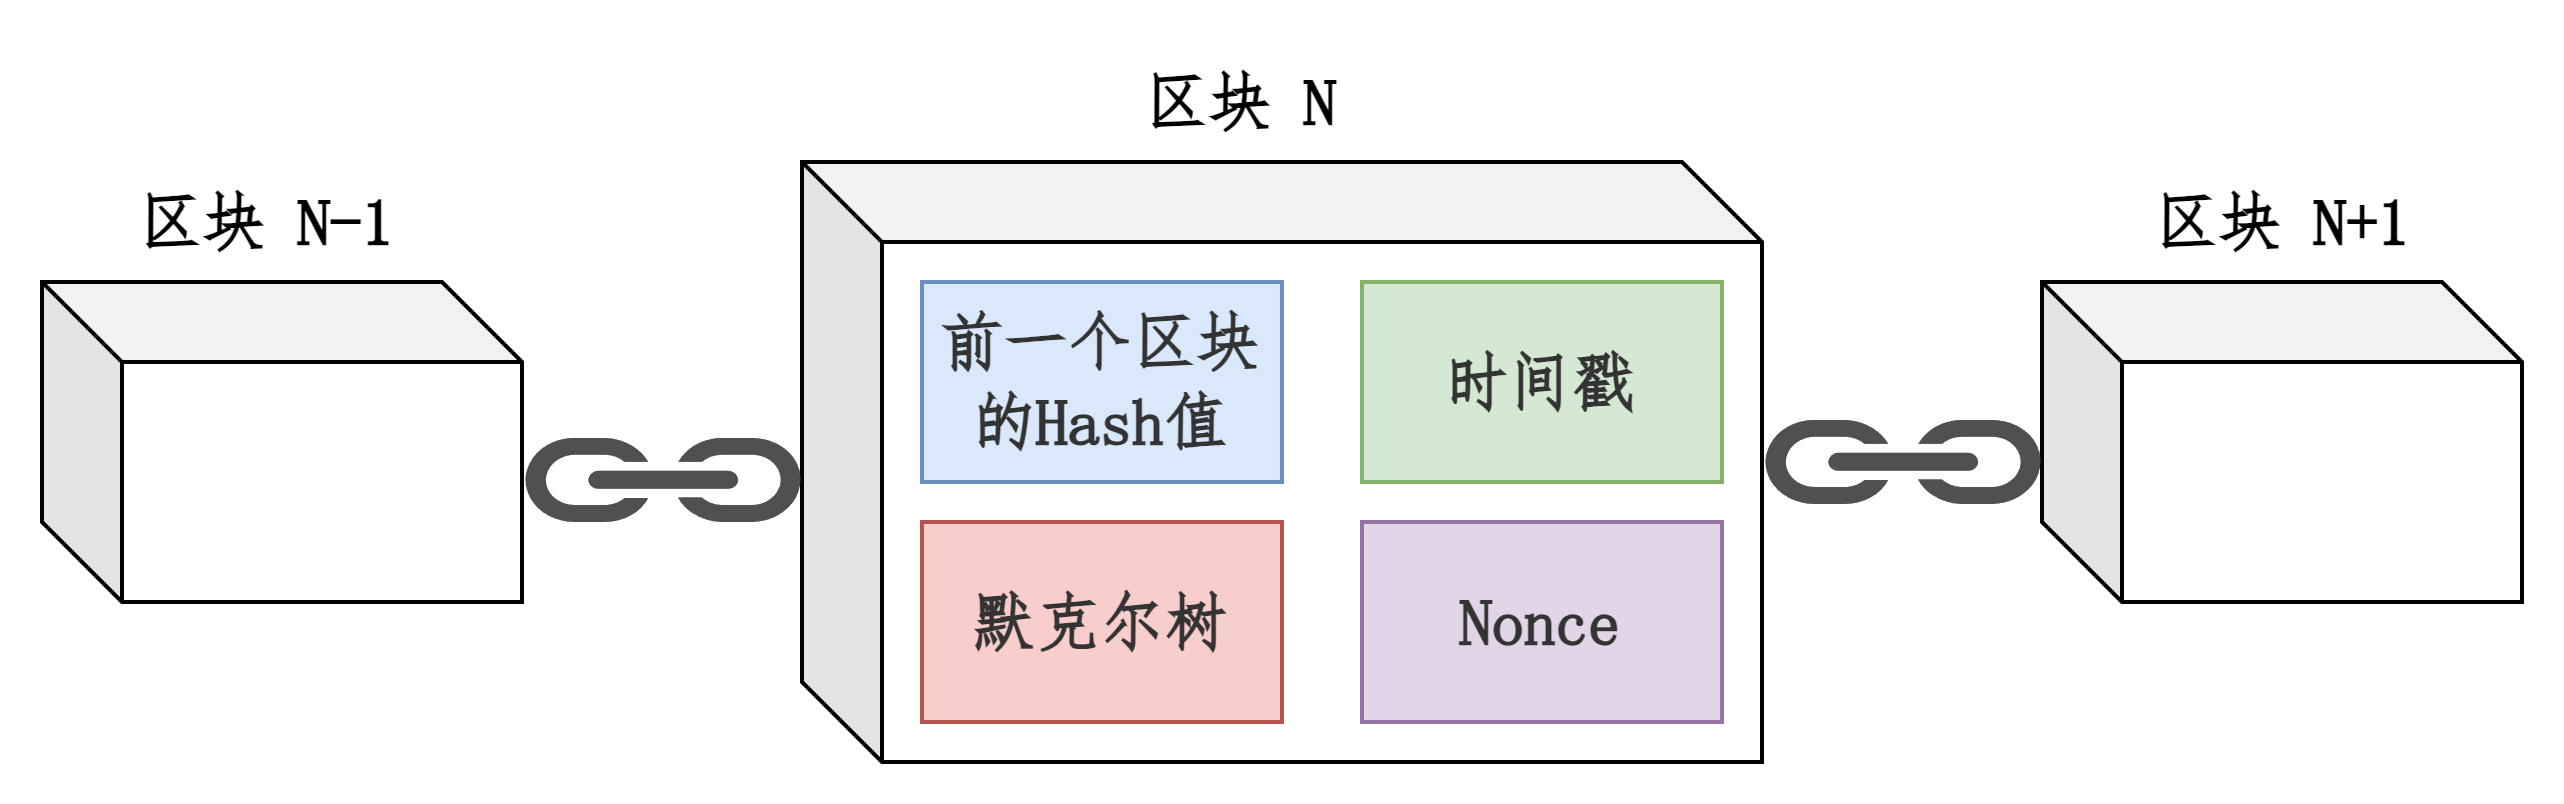
\includegraphics[width=.8\linewidth]{pictures/block_structure}
    \caption{\label{fig:block_structure}区块链的基本结构示意图}
\end{figure}
随着计算机科学和技术的不断进化,区块链这个概念已经从当初“区块”和“链”组成的数据结构,发展到基于区块链结构实现的分布式数据库技术。

狭义上来说,区块链是由众多包含信息的“区块”依次“连接”组成的链式结构,这种连接通过新的区块中包含前一个区块的唯一Hash值来实现,其基本结构如\autoref{fig:block_structure}所示,通过维护这个链式结构,区块链就成为了可以持续增长、且不可篡改的数据记录。

广义上来说,区块链代表的是基于区块链结构和点对点(Peer to Peer, P2P)网络实现的分布式数据库技术。所谓点对点网络,即不存在中心服务器为其他节点提供服务,网络中的每一个节点都可以为其他节点提供服务,节点之间可以互相交换信息。以比特币为例,在比特币系统中存在一个公共账本,记录了网络中所有的交易记录,这个账本就分布在区块链的每个区块上。每个节点都持有一份完整的账本,同时接收网络中的交易信息并进行记账,满足一定条件后,可以将自己的账本打包后添加到区块链上。

区块链的分布式存储方式与传统的分布式存储体系有两个显著的区别:首先,每个区块链节点都会以链式结构保留所有数据的完整副本,而传统的分布式存储系统通常会根据特定规则将数据切分,并在多个存储设备上进行备份。其次,区块链中的每个节点都是独立且地位平等的,它们通过共识机制来确保数据的一致性,然而在传统的分布式存储中,数据通常由中心节点同步至其他备份节点。

在区块链系统中,没有任何一个节点能够单独对账本数据进行操作,这极大地降低了由于单一记账实体被操纵或贿赂而导致的数据篡改风险。而且,由于记账节点数量众多,理论上除非超过半数的节点都遭到破坏,否则账本数据将始终保持安全,这在很大程度上确保了账本数据的安全性。

% \autoref{fig:blockchain_hierarchy}显示了区块链系统的架构模型。
% \begin{figure}[htbp]
%     \centering
%     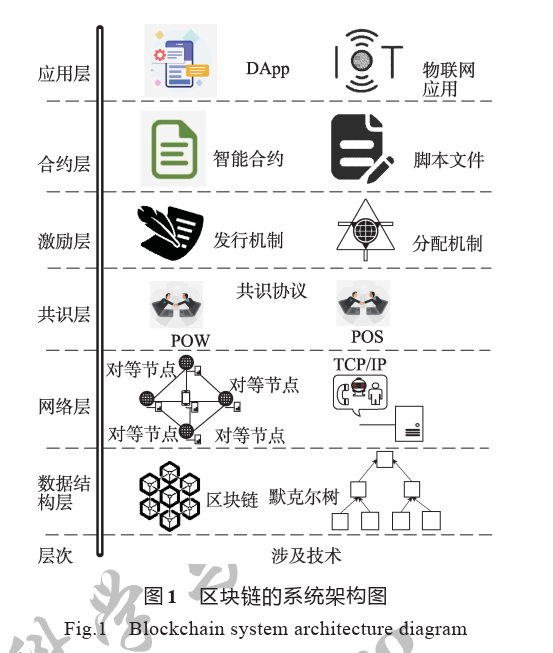
\includegraphics[width=.3\linewidth]{pictures/blockchain_hierarchy}
%     \caption{\label{fig:blockchain_hierarchy}区块链系统的架构模型}
% \end{figure}
\subsection{区块链中的关键技术}
\label{sec:区块链中的关键技术}
区块链以其安全性、高度透明和不可篡改的特性,为构建去中心化的多方协同网络提供了可信基础,被普遍认为是一项极具革命性和颠覆性的创新技术,接下来本文简要介绍一下其中的关键技术。
\subsubsection{去中心化}
    
    区块链系统的去中心化特性由P2P网络保证。与P2P网络相对应的是传统的具有中央服务器的C/S网络系统,用户接入网络后,任何与其他用户的交互行为都需要中央服务器进行转发,比如发送邮件、即时聊天、网络转账等,都需要先将请求发送到第三方软件公司的服务器上,后台程序处理这些请求并将数据发送给转账接收方或收信人。P2P网络的工作过程与上述过程截然不同。在P2P网络中,每一个网络节点既是一个用户,也能承担服务器的角色为其他节点提供服务,同时网络中的所有节点都是平等的,没有中心节点,任意两个节点之间都可以互相传输数据。在这个过程中,点对点传输既避免了可能因中央服务器宕机导致的网络瘫痪,也保证了数据传输的安全性。
    \subsubsection{一致性}
    
    去中心化特性引出了一致性问题,即如何在一个由不可信节点组成的网络中达成共识。这个问题类似于拜占庭将军问题\cite{Lamport1982TheBG},有若干支军队包围了一座城市,所有军队必须同时发动进攻才能获得胜利,但有些军队可能会选择撤退;不同军队之间只能通过信使传递消息,但有些信使可能篡改或伪造消息,因此问题就在于如何协调所有军队的进攻时机以获得最大胜利。上述问题说明了在分散、不受信任的环境中达成共识的难度。由于区块链的去中心化性质,它没有中心节点来协调其他节点,因此需要有一套规则让所有节点达成一致,以保证整个网络中只有一条“区块链”,这便是共识机制(Consensus)。工作量证明(Proof of Work,PoW)和权益证明(Proof of Stake,PoS)是最常用的实现节点共识的算法。
    \begin{itemize}
        \item 工作量证明
        
        工作量证明是区块链中最早引入的共识机制之一,也是比特币使用的共识机制。它的基本原理是通过解决数学难题,证明在创建新区块的过程中,进行了一定量的计算工作,这个过程称为挖矿(Mining)。这个数学难题是:找到一个数字(Nonce),将其结合其他固定信息计算出的哈希值能满足一定条件(如前几位为零),难点在于用户只能不断尝试不同的输入并验证结果。多个矿工同时尝试解决这个数学难题,竞争成为下一个区块的创建者,第一个成功找到符合条件的哈希值的矿工有权创建新的区块,并将这个区块广播到网络上,其他节点会验证这个区块的有效性,如果验证通过,就接受这个区块,区块链的长度此时就会增加1。尽管工作量证明被广泛应用,但由于矿工需要进行大量的无意义的计算,因此该方法最显著的缺点就是能源消耗\cite{wangdan}。这也导致了对更环保的共识机制的不断探索,如接下来要介绍的权益证明等。
        \item 权益证明
        
        权益证明试图解决工作量证明算法中的能源消耗问题。在权益证明算法中,拥有更多加密货币的用户创建的新区块更容易被接受,这个算法假设拥有更多加密货币的用户更倾向于维护整个网络的稳定\cite{zheng2017overview},这与现实生活中的股份制较为相似,持有股份更多的人拥有更大的话语权。但在实际情况中,这种算法更容易产生垄断情况,即富有的人通过记账获得奖励后会变得更富有,因此也有一些变种形式的权益证明法被提出,如委托权益证明(Delegated Proof of Stake,DPoS)。
        \item 委托权益证明
        
        委托权益证明由权益证明法改进而来,其原理是:先根据持有的加密货币数量选出一些代表用户去竞争记账权,每个用户可以进行投票,选出更适合记账的用户代表,如果拥有记账权的用户不称职,就随时有可能被投票出局,这在一定程度上改善了权益证明法的缺点。
    \end{itemize}
    \subsubsection{安全性}
    
    区块链主要依靠加密技术来保证数据的安全性。前一个区块的数据和哈希值决定了下一个区块的哈希值,倘若区块中的数据被篡改,无论篡改的数据量大小如何,都会导致最终生成的哈希值与原始数据生成的哈希值截然不同。同时,在共识机制的作用下,被篡改的数据不会得到其他节点的承认,除非攻击者能操控整个网络中超半数的节点,而这显然是不可能的。除此之外,密码学中的非对称加密算法也能保障区块链的安全性。非对称加密算法使用一对密钥:公钥和私钥,公钥是公开的,私钥只有用户本人持有。用户可以使用私钥对交易进行签名,其他用户可以使用该用户的公钥对交易进行验证,这便是数字签名,它确保了交易的真实性和不可抵赖性。
    


\section{以太坊}
\label{sec:以太坊}
\subsection{以太坊简介}
\label{sec:以太坊简介}
在比特币项目获得巨大成功后,有一些开发者开始思考能否将区块链技术拓展到更多的应用场景,原因在于比特币项目的本义就是使用数字货币存储价值,其智能合约语言的局限性使得比特币系统难以扩展出其他能力。2013年底,维塔利克·布特林提出了在区块链上运行图灵完备的应用程序的设想,为此他提出了以太坊项目。以太坊也有其专属的电子货币——以太币,除了基本的金融交易,以太坊还支持用户开发部署自己的智能合约,创造各种去中心化应用程序,因此以太坊也被称为“下一代电子货币和去中心化应用平台”。\autoref{fig:以太坊架构图}展示了以太坊平台的架构示意图。下面简要介绍一下以太坊的主要特点。
\begin{figure}[htbp]
    \centering
    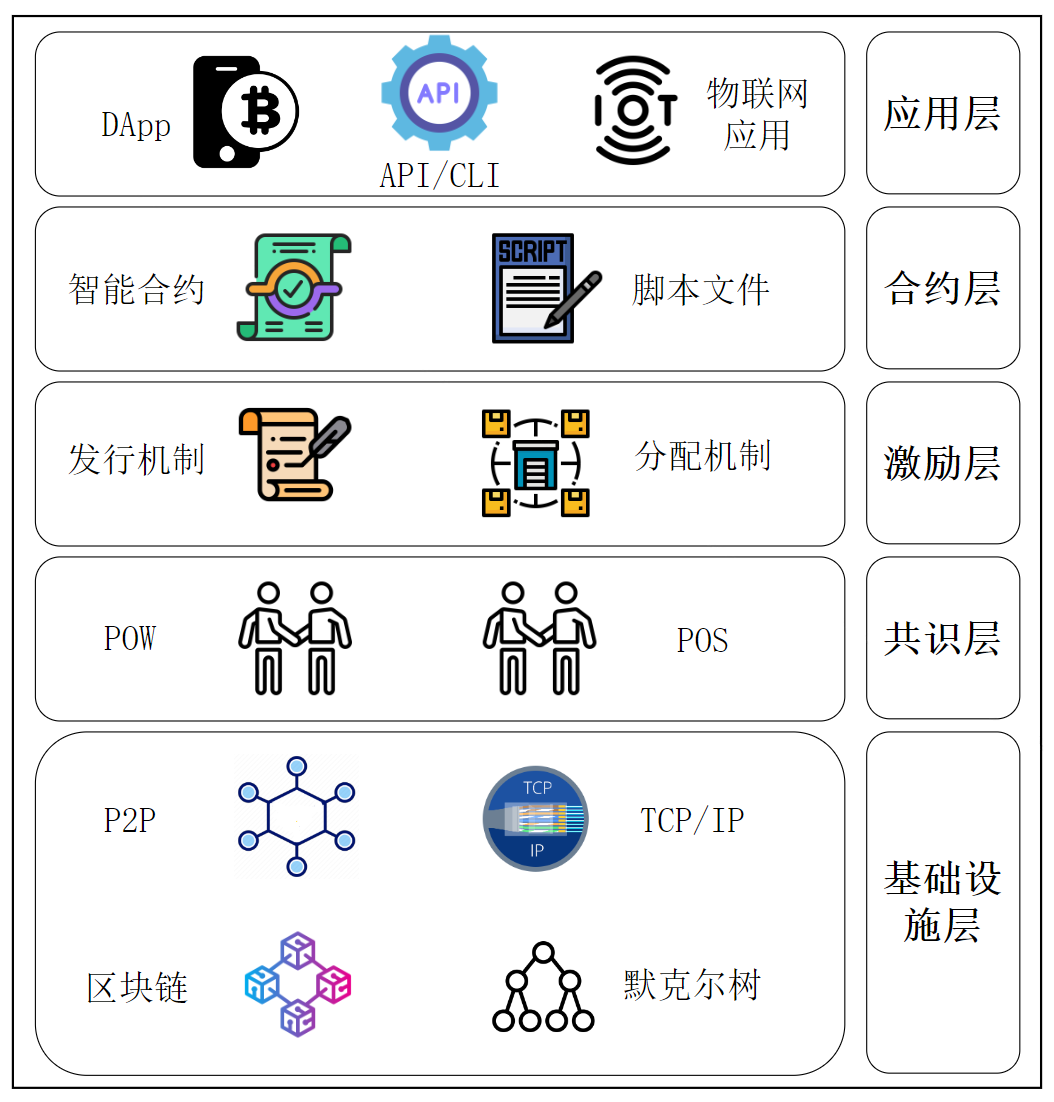
\includegraphics[width=.6\linewidth]{pictures/以太坊架构图final.png}
    \caption{\label{fig:以太坊架构图}以太坊平台的架构示意图}
\end{figure}
\subsubsection{账户}
    
    比特币系统作为分布式记账平台,任何人都可以通过遍历交易记录推断出用户的余额,而以太坊针对此提出了账户的概念。账户可以记录多种类型的信息,如用户的余额、智能合约代码等,以太坊中共有两种账户:外部账户(Externally Owned Account,EOA)和合约账户(Contracts Account)。\autoref{fig:account}显示了以太坊账户的基本结构。
    \begin{itemize}
        \item 外部账户
        
        外部账户类似现实世界中的银行账户,是以太币拥有者的账户,记录了用户的余额和发送交易的数量等信息。外部账户可以互相转账,也可以调用合约账户以执行智能合约代码。外部账户与一对密钥绑定,公钥经过计算后得到的哈希值作为账户地址被公开,其他用户可以通过此地址进行转账;私钥由用户本人持有,可以对该外部账户进行完全访问和控制,该账户发送的每个交易都需要使用私钥进行签名,其他账户可以使用公钥进行验证以实现防伪。
        \item 合约账户
        
        合约账户即智能合约账户,主要功能就是存储智能合约代码。用户编写好智能合约代码并部署到以太坊时,合约账户就会被创建。合约账户也可以持有和接收以太币,用于支付合约代码的存储和执行所消耗的网络资源。和外部账户不同的是,合约账户只有公钥没有私钥,它们不能主动发起交易,只能被外部账户调用。
        
    \end{itemize}
    \begin{figure}[htbp]
        \centering
        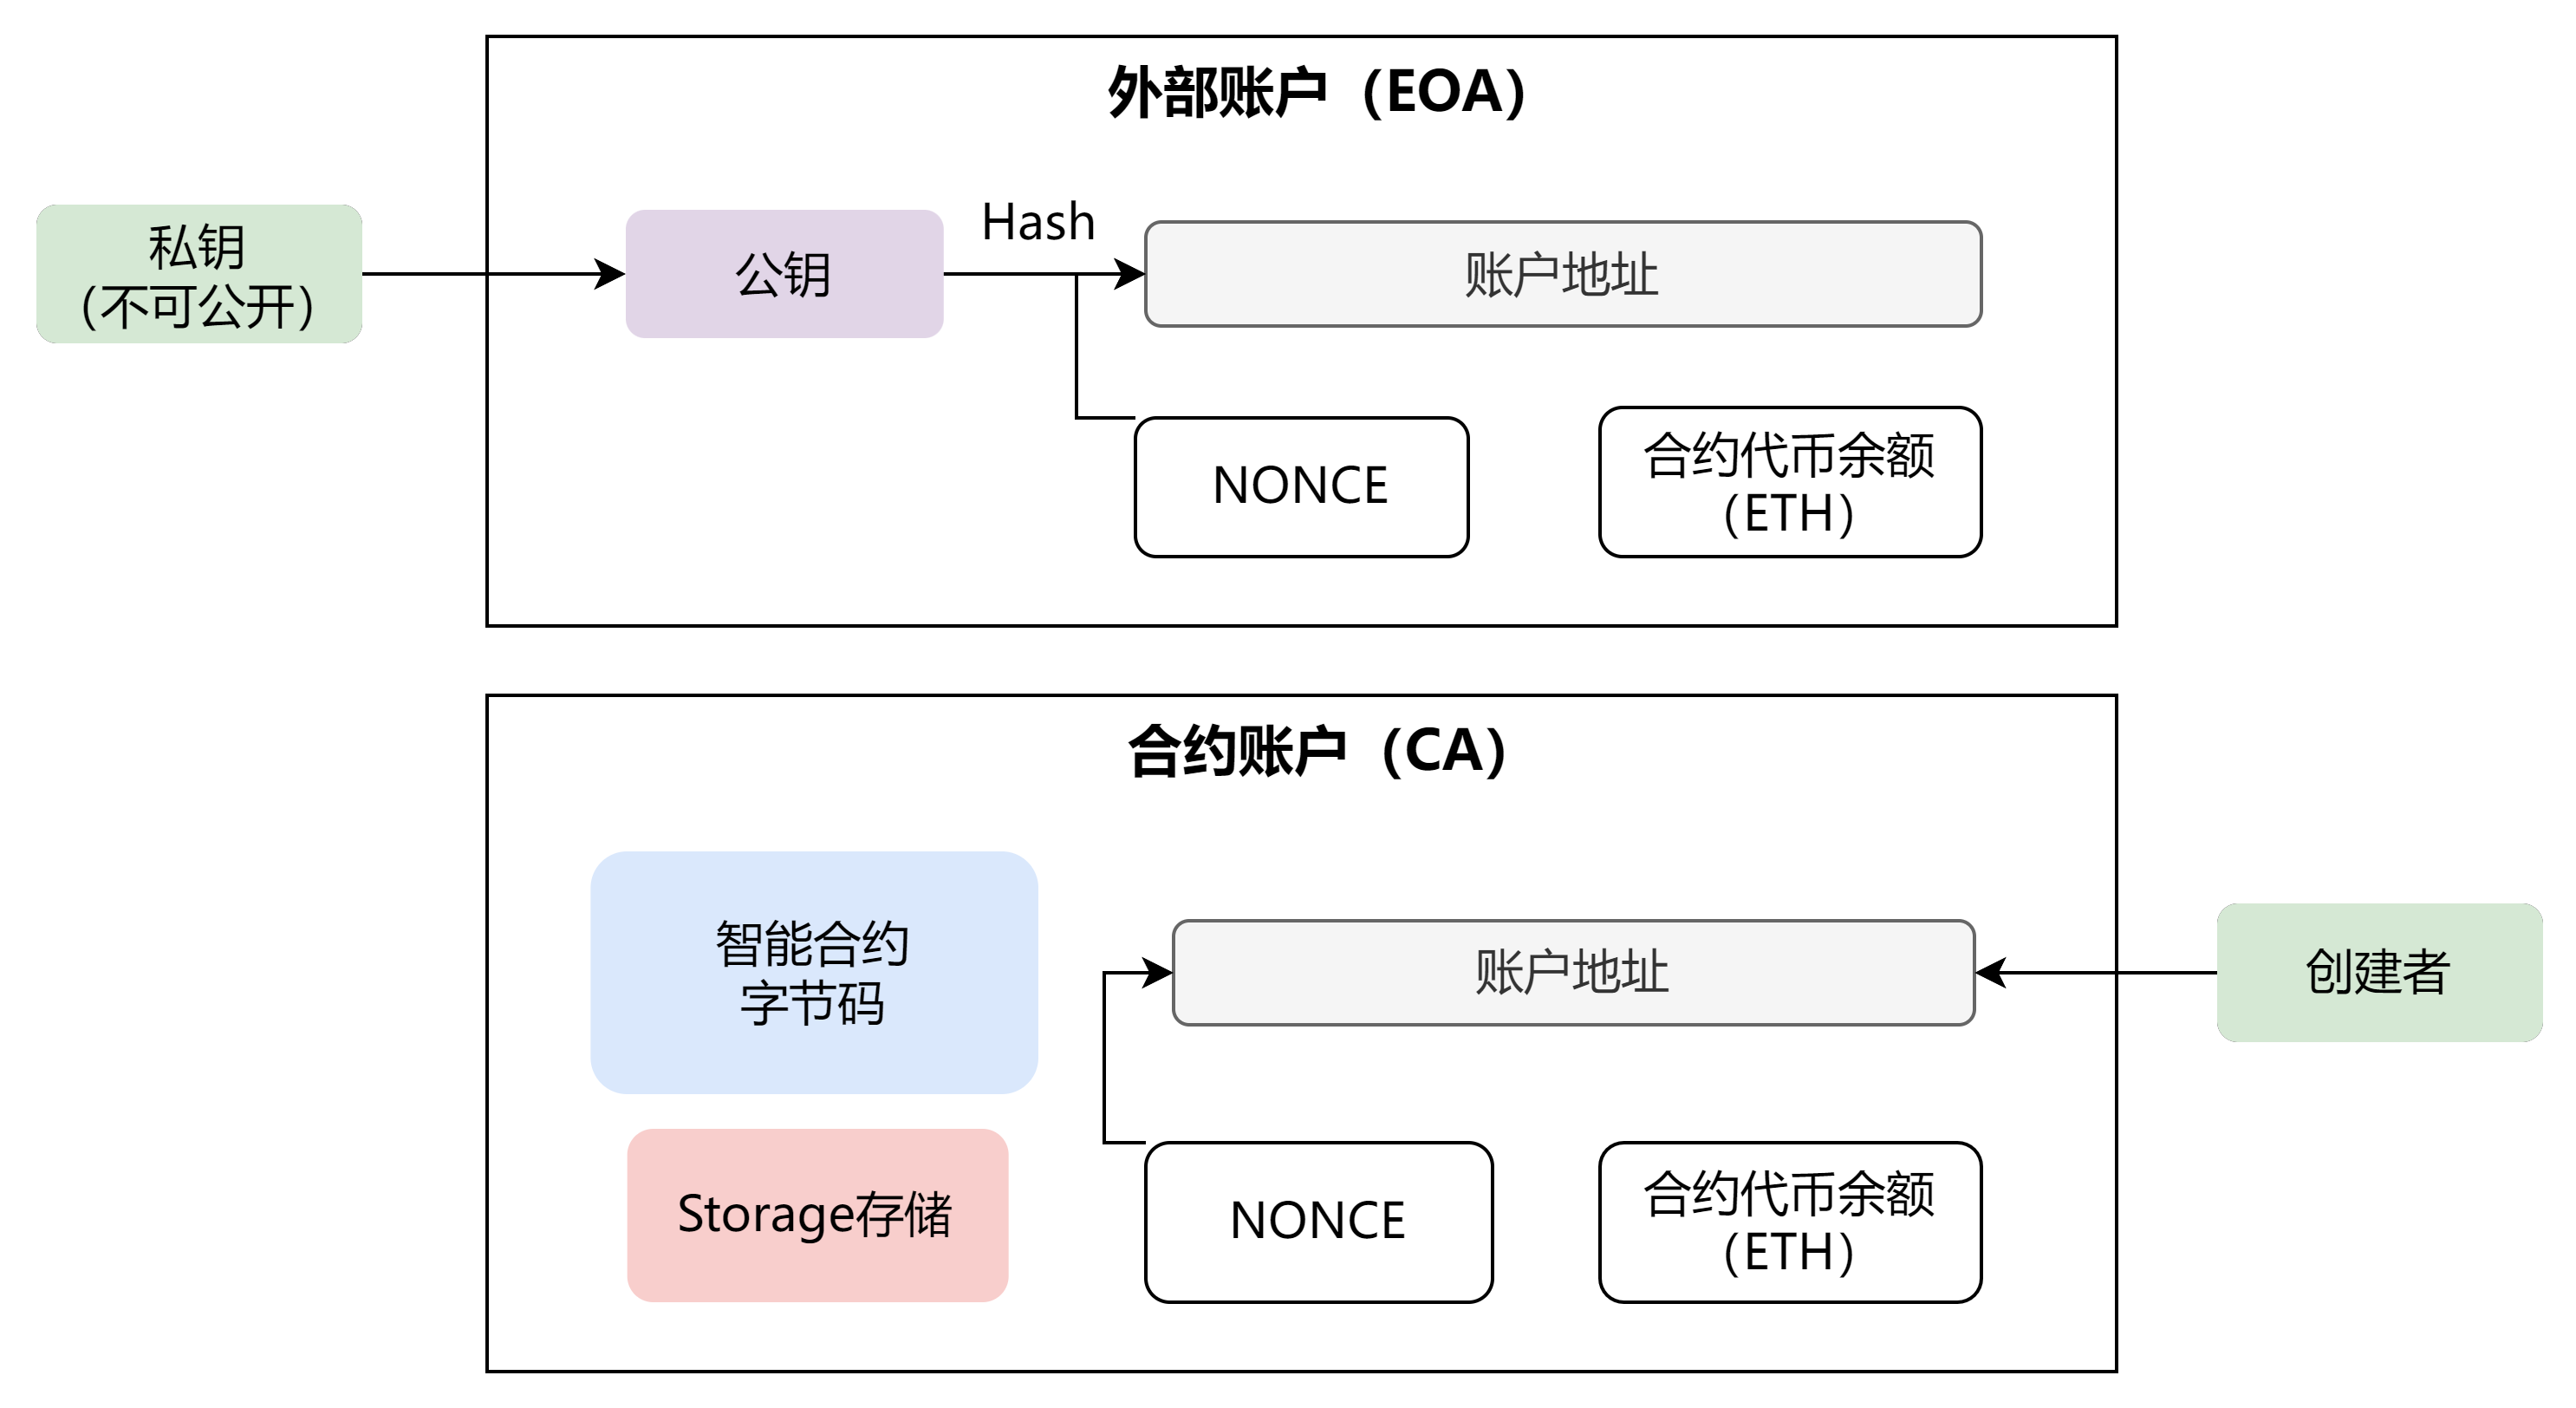
\includegraphics[width=.7\linewidth]{pictures/account}
        \caption{\label{fig:account}以太坊两种账户的基本结构}
    \end{figure}
\subsubsection{交易}
    
    交易是用户在以太坊网络上交互的主要方式,通过交易,用户可以进行转账、部署或调用合约。需要注意的是,交易只能由外部账户发起,并且在发送交易前,用户需要缴纳一定的手续费,通过以太币方式进行支付,这个费用被称为“Gas”。发起一笔交易需要指定一些关键信息,如交易的发送方和接收方地址、发送的以太币数量,可以消耗的最大Gas数量等。目前以太坊支持三种交易:
    1)转账:将以太币发送到另一个账户,可以是外部账户也可以是合约账户;
    2)部署合约:将编写好的智能合约代码部署到以太坊网络上;
    3)执行合约:使用指定参数调用已部署的智能合约。

    交易是以太坊中的关键技术,它在网络中实现了价值传递,促进了金融交易和去中心化应用的发展。
\subsubsection{去中心化应用}
    
    任何人都可以在以太坊上部署自己的去中心化应用(Decentralized App,DApp),去中心化应用与中心化应用相对,前者没有固定的中央服务器,而是借助点对点网络实现分布式存储和计算。去中心化应用由前端和后端构成,前端是用户界面,可以由任何语言编写,用户可以通过它与应用程序进行交互;后端则是部署在区块链上的智能合约,其中定义了应用程序的执行逻辑\cite{lileixiao}。去中心化应用依托区块链技术,具有去中心化、开源、自治和透明的特点,可以为用户提供更高的可靠性和安全性,DApp的应用领域也将随着区块链技术的发展而不断扩大。


\subsection{以太坊运行机制}
\label{sec:以太坊运行机制}

\subsubsection{以太坊虚拟机}
    
    以太坊虚拟机(Ethereum Virtual Machine,EVM)是智能合约运行的基础环境,也是以太坊的核心组件。以流行的Java编程语言进行类比,Java语言编写的程序运行在Java虚拟机上,Solidity语言编写的智能合约则运行在EVM上。EVM的基本结构如\autoref{fig:evm2}所示。
        \begin{figure}[htbp]
            \centering
            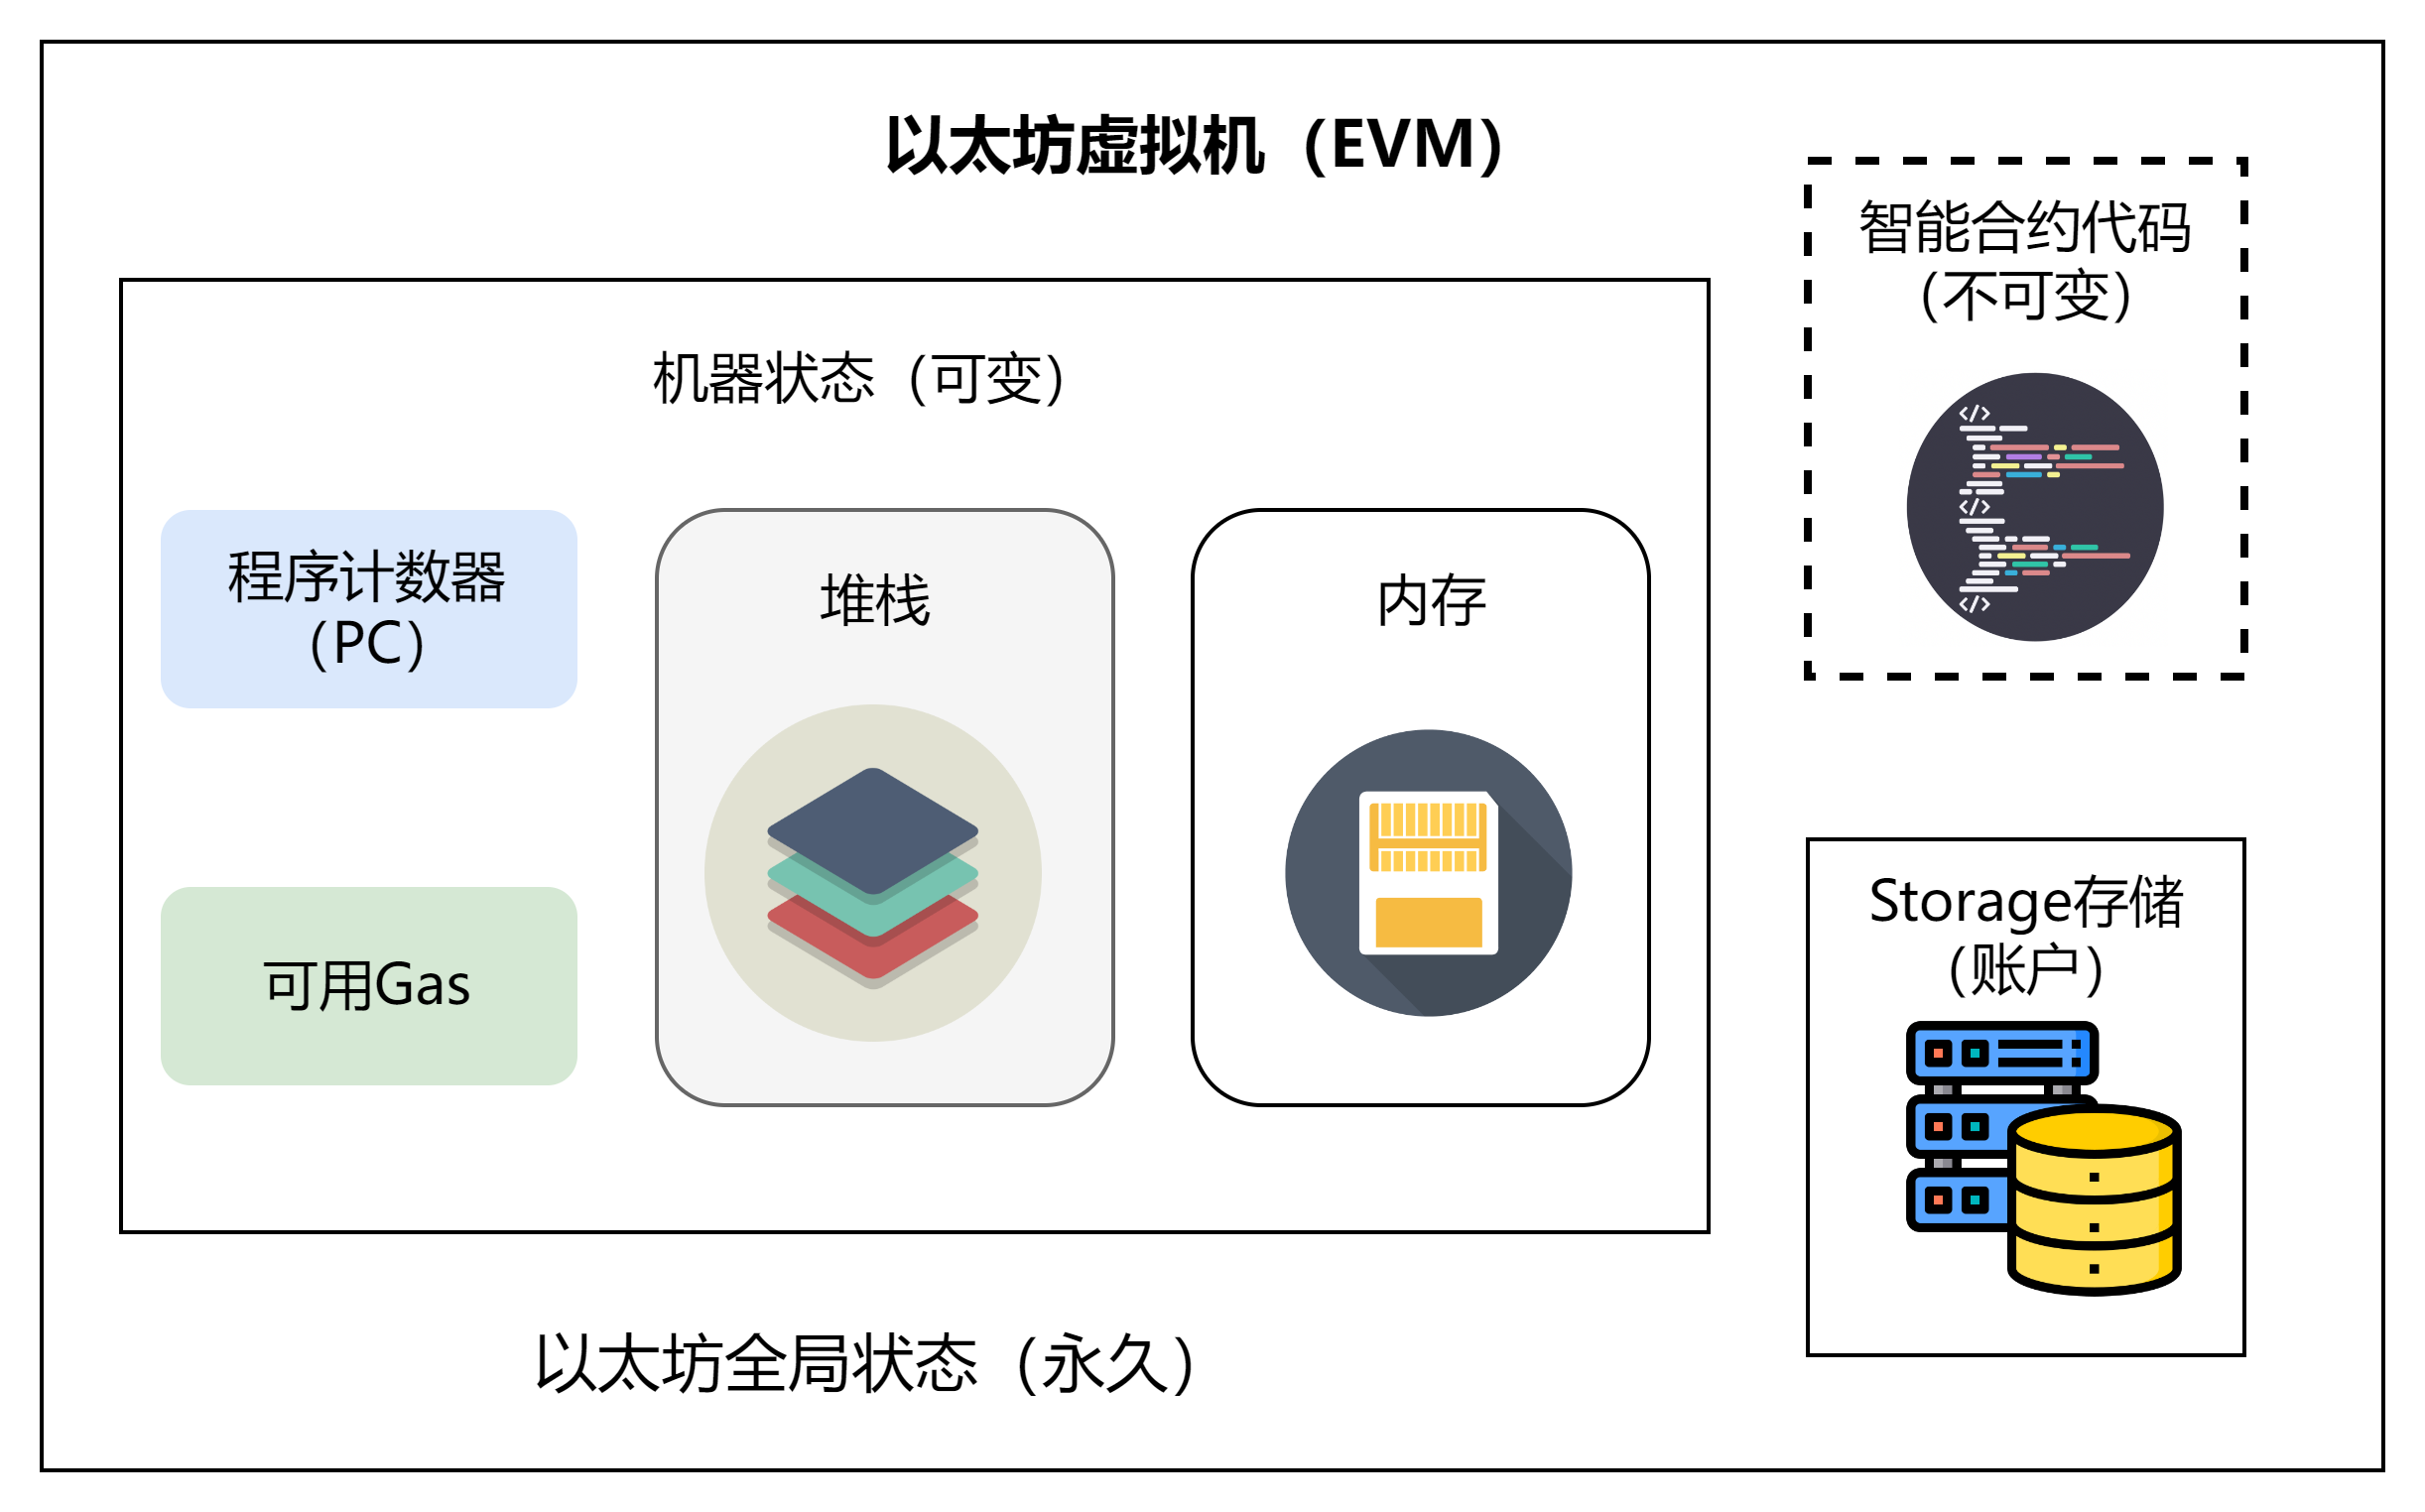
\includegraphics[width=.7\linewidth]{pictures/evm2}
            \caption{\label{fig:evm2}以太坊虚拟机的基本结构}
        \end{figure}

    EVM采用基于栈的架构,具备图灵完备性,允许开发者编写包含逻辑判断和循环结构的复杂智能合约。正如Java虚拟机并不能直接执行Java程序,需要使用相关工具将Java程序转换为字节码,然后交由Java虚拟机执行。同样地,智能合约也需要被转换成字节码才能交由EVM执行。字节码由一系列操作码组成,操作码(OpCode)是定义以太坊虚拟机操作的指令集,涵盖加法、乘法、逻辑运算等各种特定操作。智能合约源代码经过编译转化为字节码,然后部署到以太坊区块链上,等待被某个节点上的EVM调用执行。

    EVM支持多种编程语言,其中以Solidity最为广泛使用。Solidity是一种专门为以太坊智能合约设计的高级编程语言,它类似于JavaScript,但具有更强的安全性和适应性,可以编写复杂的智能合约逻辑。由于EVM执行的是字节码,所以理论上可以使用任意高级编程语言编写智能合约,然后使用特定的工具将其编译为字节码,这种灵活的编程框架使得以太坊成为开发者构建去中心化应用(DApps)的理想平台\cite{chen2020understand}。

    EVM的另一个重要特性是其状态转换功能。每个智能合约都有一个与之关联的状态,EVM通过在执行智能合约时更新状态来实现对区块链上数据的更改。这种状态转换通过交易驱动,一旦交易被矿工节点确认,智能合约的状态变化就会被永久记录在区块链上。

    总体而言,EVM作为以太坊的核心组成部分,为开发者提供了一个安全、可信的智能合约执行环境,推动了去中心化应用的发展,同时其Gas计费模型和状态转换机制为以太坊网络的稳定性和可扩展性奠定了基础。   
    
\subsubsection{Gas机制}
    
    智能合约部署到以太坊之后就可以被任何人调用,而调用执行智能合约会消耗矿工的计算资源和网络资源。想象以下场景:有人发送了一笔交易,其中通过构造死循环调用了某个智能合约,当某个矿工接收到这笔交易并决定执行它时,他就会在自己的机器上无限调用某个智能合约,最终导致矿工的系统资源被耗尽,并可能导致以太坊网络阻塞。为了避免上述情况的发生,发送交易的一方需要为此笔交易支付手续费,从而限制智能合约执行时的资源消耗。

    由于以太币的价格是随时变动的,不能直接使用以太币作为计费单位,因此以太坊引入了Gas机制。以太坊黄皮书中定义了详细的Gas消耗规则,EVM会根据这些规则计算出执行一个合约需要消耗的Gas总量。一个Gas的价格不是固定的,Gas与以太币之间存在兑换关系\cite{tuliangqiong}。在发送交易时,发送方需要设置两个关键参数:gasLimit和gasPrice。gasLimit表示执行本次交易可供消耗的Gas数量的上限,gasPrice表示发送方定义的Gas的单价,最终发送方为本次交易支付的手续费总额是:交易消耗的Gas数量与gasPrice的乘积。倘若本次交易消耗的Gas数量超过了gasLimit时,EVM就会报告异常从而拒绝继续执行该交易,反之,当交易执行完成后,多余的Gas会返还给发送方。

    Gas的引入不仅限制了复杂操作的数量,也防止了恶意代码无限消耗计算资源。这种基于Gas的计费模型旨在确保网络的公平性和稳定性,然而也可能存在安全风险。攻击者可能通过滥用这一机制导致程序异常,进而触发合约的安全漏洞,影响其正常执行。因此,在智能合约的设计和使用过程中,需要充分考虑这些潜在的安全问题。

\section{智能合约}
\label{sec:智能合约}
\subsection{智能合约简介}
\label{sec:智能合约简介}
智能合约是一种计算机程序,可以由高级编程语言(如Solidity)编写,并在预定的条件被触发时自动执行。智能合约的概念最早由密码学家尼克·萨博(Nick Szabo)在1994年提出,但直到2014年以太坊诞生,智能合约才真正得到实际应用并开始流行起来。

智能合约的特点在于它的自动执行性、透明性和不可篡改性。首先,智能合约的自动执行性显著降低了传统合同执行过程中的时间和成本。在智能合约中,一旦预设条件得到满足,合约便自动执行,无需第三方介入。这种机制不仅提高了效率,还增加了执行的可靠性,避免了人为操作过程中的失误。其次,透明性和不可篡改性是智能合约的另两大特点。由于智能合约存储于区块链上,任何人都可以查看合约条款和执行情况,这种透明性保证所有相关方能得到公平对待。同时,一旦智能合约被部署到区块链上,它就不能被更改或删除,这为合约的可信度和安全性提供了强有力的保障。

这些特性使得智能合约在许多领域都有潜在的应用。例如,在金融交易中,智能合约可用于自动支付;在供应链管理中,智能合约可以自动追踪和验证商品的来源;在房地产交易中,智能合约可以自动完成物业的买卖和转移。
如今智能合约已经成为区块链技术的不可或缺的组成部分,也是推动区块链技术应用的关键因素。正是智能合约的出现,区块链技术的应用才不再局限于数字货币,为实现去中心化的数字社会提供了可能。

由于智能合约可有多种高级编程语言编写,且可以运行在多种区块链应用上,因此如无特殊说明,本文中讨论的智能合约均指由Solidty语言编写、并运行在EVM上的智能合约。
\subsection{智能合约漏洞}
\label{sec:智能合约漏洞}
由于智能合约自动执行和不可更改的特性,一旦有合约中的漏洞被黑客利用并且转移了资金,那么几乎是没有办法逆转交易的\footnote{唯一的方法是硬分叉,详见https://corporatefinanceinstitute.com/resources/cryptocurrency/hard-fork/},因此对智能合约漏洞检测的研究一直都很受欢迎。智能合约从编写、部署、运行的各个生命周期都可能引入安全漏洞,以次为依据可以将智能合约安全漏洞分为三个层面:Solidity层面、EVM层面和区块链层面。已有大量工作提出了很多智能合约漏洞类型,随着技术发展和版本更迭,也有一些类型的漏洞被修复。参考DASP发布的十大智能合约漏洞\cite{dasp10},\autoref{tab:smart_contract_vulnerabilities}展示了一些主要的智能合约安全漏洞类型。
\begin{table}[htbp]
    \caption{\label{tab:smart_contract_vulnerabilities}现有的智能合约漏洞检测方法}
    \small
            \renewcommand{\arraystretch}{1.5}
        \begin{tabularx}{\linewidth}{cp{3cm}<{\centering}X<{\centering}X<{\centering}}

    \hline
    \multicolumn{1}{l}{漏洞层级}    & 漏洞类型   & 漏洞原因                              & 安全问题    \\ \hline
    \multirow{5}{*}{Solidity层面} & 访问权限控制 & 未使用或使用了错误的访问权限修饰符,以及使用了tx.origin  & 函数或变量可以被任意用户或变量调用 \\
                                & 算术漏洞   & 整数上溢出或下溢出                         & 运算结果错误或合约执行崩溃 \\
                                & 未检查的调用 & 对可能失败的调用未进行异常捕获处理                 & 合约执行崩溃 \\
                                & 重入漏洞   & fallback函数递归调用了外部合约               & 无法安全使用合约代币 \\
                                & 拒绝服务   & 意外情况导致合约主动终止运行,如revert指令、Gas超出上限等 & 合约无法被正常调用 \\ \hline
    EVM层面                       & 短地址    & 合约地址长度不符合要求而被EVM拒绝执行              & 合约无法被正常调用 \\ \hline
    \multirow{3}{*}{区块链层面}      & 时间戳注入  & 矿工恶意修改区块的时间戳                      & 无法安全使用合约代币 \\
                                & 抢先执行   & 通过增加Gas来抢占相同交易的执行时机             & 交易竞争导致合约无法被正常调用 \\ \hline
        \end{tabularx}
\end{table}
下面详细介绍一些重要的智能合约安全漏洞类型。
\begin{enumerate}[label=(\arabic*)]
    \item 访问权限控制
    
    访问权限控制是指在面向对象编程中,一个对象的函数或变量是否可以被本对象或外部对象访问。除了基本的访问修饰符public和private外,Solidity还支持external和internal修饰符,表示该函数或变量是否可以被本合约和其他合约访问。同时Solidity还支持进一步对调用者的身份进行限制,比如onlyAdmin和onlyOwner修饰的函数只允许被管理员角色或用户角色调用\cite{grishchenko2018semantic}。
    \item 算术漏洞
    
    算术漏洞主要是指整数上溢出或下溢出。整型变量根据其占用字节数只能存储一定范围内的值,如果要存储的值超出范围的上限或下限都会导致原数值被截断,只存储原数值二进制表示的低位部分。由于存储了错误的数值,必然会造成合约执行逻辑上的错误。
    \item 未检查的调用
    
    智能合约可以调用执行其他合约,根据调用结果执行相应的逻辑。这个过程可能会由于编程错误或遭受攻击而导致失败,如果不对调用失败后的异常进行处理,就可能会进一步导致合约无法被正常执行。比如使用call或delegatecall函数调用了未知地址的合约可能会导致恶意代码被执行,或者通过循环调用一些失败的合约发动拒绝服务攻击,这些问题都可以通过编程的方式在一定程度上避免,比如在调用前对被调用合约的地址进行检查,以及在调用后对可能出现的各种结果进行处理\cite{zhang2022zh}。
    \item 重入漏洞
    
    重入漏洞是智能合约中非常著名的漏洞之一,发生于2016年的大名鼎鼎的The Dao攻击正是利用了这一漏洞。重入漏洞源于Solidity中独特的回调机制。每个智能合约中都有一个fallback函数,当外部账户或其他合约向该合约转账或调用不存在的函数时,fallback函数就会被虚拟机调用。攻击者可以在恶意合约的fallback函数中从被攻击合约转账,由于上述机制,fallback函数会不断被调用,被攻击合约的余额也会不断被转移,直到余额为0或者交易消耗的Gas达到了上限。
    %%%%%%%%%%%%%%%%%%%%%%
    % \item 拒绝服务
    
    % 拒绝服务(Denial of Service,DoS)一直以来都是软件工程领域最常见的漏洞之一。在以太坊中,合约执行所消耗的Gas有一个上限,如果一个交易花费的Gas超过这个上限就会导致合约执行失败,当合约执行耗时计算或受到恶意消耗Gas的攻击时就可能导致Gas达到这个上限,进而导致该合约无法正常提供服务。
    % \item 短地址
    
    % 短地址漏洞源于以太坊虚拟机对字节码的自动补全机制。以太坊标准规定智能合约地址值必须为固定长度的20字节,如果不足就需要截取相邻的二进制位以满足地址长度的要求,同时在字节码的末尾补0以满足整个编码数据长度的要求,这会导致原二进制串中数据段的值被修改,从而产生错误的逻辑。例如ERC20智能合约中定义的transfer转账函数,其参数为20字节的地址和32字节的转账金额,攻击者可能故意提供19字节的地址和32字节的转账金额,由于地址长度不足20字节,转账金额数据的首个字节会被截断成为地址值的一部分,同时在转账金额的末尾填充1字节的0,这也意味着转账金额左移1字节后增大了256倍,因此实现盗窃用户资产的目的。短地址攻击的应对方法就是在调用转账函数时,对转账地址进行严格的校验,避免触发字节码的自动补全机制。
    % \item 时间戳注入
    
    % 以太坊中区块的时间戳由打包这个区块的计算机时间决定,整个区块中的所有交易在执行时都可以通过调用block.timestamp获得时间戳,如果在智能合约的条件判定部分使用了时间戳,那么就很有可能被矿工恶意篡改其计算机时间,以达到对其有利的目的。为了应对这个漏洞,合约中可以不使用时间戳作为重要逻辑的判定条件,或者使用第三方服务(如Oraclize)获取随机值作为判定条件。
    %%%%%%%%%%%%%%%%%%%%%%%%%%%%%%%%%
    % \item 抢先执行
    
    % 在以太坊中存在一个交易池(Mempool)记录了所有等待被打包的交易,交易池会被广播到整个以太坊网络供获得打包权的矿工打包成一个新的区块。然而交易池中的交易被执行的顺序不是固定不变的,它由交易发起方提供的Gas多少决定,交易发送方提供的Gas越多,该交易就越可能被先执行。攻击者如果从交易池中发现了一些有价值的信息,那就可以提交相同的交易但附带更多的Gas,那么攻击者发送的交易就会先被矿工执行,从而抢占了相同交易的执行时机以获取某些利益。
\end{enumerate}
\subsection{智能合约运行时崩溃}
\label{sec:智能合约运行时崩溃}
智能合约作为计算机程序,也可能会在执行过程中发生异常从而导致执行失败。有研究显示\cite{reducing2020},截止2020年以太坊上有4.9\%的交易执行失败,这些执行失败的交易不会改变以太坊全局状态,这是对计算资源的浪费。而且,由于区块链的不可篡改性,所有处理过的交易,包括执行失败的交易都会永久存储在区块上,浪费了存储空间。根据Siwapol等人的研究结果\cite{reducing2020},截止2020年,以太坊平台已经为执行失败的交易支付了约2800万美元的交易费和1210亿美元的区块奖励。

智能合约执行失败的原因多种多样,但总体上可以分为两类:内部因素和外部因素。内部因素是指合约在开发过程中引入的逻辑或算法错误,通常源于开发者疏忽、测试不足或复杂的合约逻辑。其次,外部环境也可能影响智能合约的执行结果。区块链作为分布式系统,它依赖多个节点的合作执行合约,节点间的通信或同步问题,以及网络拥堵、攻击或其他技术问题均可能导致合约执行失败。

在以太坊中,虚拟机在执行合约过程中因运行时异常而停机就意味着合约执行失败,白皮书中列出了五种以太坊虚拟机可能抛出的运行时异常:
\begin{enumerate}[label=(\arabic*)]
    \item Gas不足
    
    Gas不足(Out-of-Gas)是指在合约执行过程中,交易发送方提供的Gas被耗尽,导致该异常的原因通常是:交易发送方在发送交易前提供的Gas过少,或者代码编写不当,比如存在无法结束的循环或者过多耗时的操作等。
    \item Reverted
    
    REVERT是拜占庭硬分叉中引入的虚拟机操作码,通常由开发者用于验证合约的输入或状态是否符合要求,如检查合约的所有权、账户余额或时间等。为了保证交易的原子性,当遇到REVERT操作码时,虚拟机会撤销本次合约执行过程中所有的状态更改,就好像本次交易从未被执行过一样。与其他运行时异常不同,REVERT是一种安全友好的结束合约执行的方式,它会将未消耗完的Gas退还给交易发送方。
    \item 无效操作码
    
    无效操作码(Invalid Opcode)表示虚拟机从合约字节码中解析出的操作码不与任何已知的操作码匹配,或者操作码的参数个数或值的范围不符合规范。还有一种情况,当智能合约使用的Solidity版本与EVM不兼容时,虚拟机就会抛出无效操作码的错误。
    \item 无效跳转
    
    无效跳转(Invalid Jump)是指跳转操作码的目标地址不合法,比如调用一个在合约中不存在的函数。
    \item 堆栈溢出
    
    堆栈溢出(Stack Overflow/Underflow)包含堆栈上溢出和下溢出。上溢出是指虚拟机在运行过程中栈帧数目达到了上限,虚拟机标准规定栈帧数目的上限是1024,如果超过这个上限,就会出现堆栈上溢出错误。这往往发生在递归调用中,递归函数中的退出条件永远无法满足,解决方法就是正确编写递归程序。堆栈下溢出的情况非常少见,它是指在空堆栈上执行POP操作码而导致的错误,但一般不会出现这种情况,除非对智能合约编译后的字节码进行刻意修改。
\end{enumerate}
% 区块链的不可篡改性为软件工程带来了新的挑战,一旦智能合约被部署到区块链上,合约的源代码就无法被修改,任何代码中的错误都会对整个区块链产生持久影响。